\chapter{Preliminaries}
\textit{This chapter refers to (and summarizes) my Master 1 project. Concepts and definitions are essentially inspired by the chapter 10 of the book ``Principles of model checking'' \cite{PMC}, the chapter ``Model checking probabilistic systems'' of the Mickael Randour course called ``Formal verification of computer systems'' \cite{MRV} as well as the article ``Variations on the shortest path problem'' \cite{DBLP:journals/corr/RandourRS14a}.} \\

Before studying the different multi-objective problems in a \textit{Markov decision
process} and defining \textit{strategies} that solve such problems, we will introduce some fundamental concepts that define the area of the subject.
Actually, we will be interested to know some measurements related to the cost of \textit{paths} of Markov decision process and these measurements can not be computed without defining a probability measure on these paths.
So, first of all, we need to define what are \textit{Markov chains}. Indeed, these
stochastic models are essential to measure the probability of \textit{paths} of a Markov decision process.

\section{Markov chains}
\begin{definition}[\textbf{Discrete-time Markov chain}]
  A \textit{(weighted) discrete-time Markov chain} (denoted by \textbf{MC}) is a stochastic model defined by a tuple $\mathcal{M}=(S, \Delta, w, AP, L)$ where
	\begin{itemize}
		\item $S$ is a set of states,
		\item $\Delta: S \times S \rightarrow [0,1] \cap \mathbb{Q}$ is a  \textit{transition function} such that \[\forall s \in S, \sum_{s' \in S}\Delta(s, s')= 1\]
		%\item $d_0:S \rightarrow [0,1]$ est la distribution initiale telle que \[\sum_{s \in S}d_0(s)= 1\] (à noter que dans le cadre de ce document, la distribution initiale peut être omise, et dans ce cas, $\forall s \in S, d_0(s) = \frac{1}{|S|}$).
		where $\Delta(s, s')$ describes the probability that the system goes from state $s$ to state $s'$ in one transition,
    \item $w : S \times S \rightarrow \mathbb{N}_0$ %est la fonction
        %de poids associant à chaque transition un coût strictement positif.
      is a weight function that links a strictly positive cost to each transition,
    \item $AP$ is a set of atomic propositions, and
    \item $L : S \rightarrow 2^{AP}$ is a labeling function.
	\end{itemize}
  \textit{Note }: $AP$ and $L$ can be ommited. In that case, we will consider that $AP = S$ and $L$ is the natural labeling of each state, i.e., for all $s \in S$, $L(s) = \{s\}$
\end{definition}

\begin{property}
  Let $\mathcal{M} = (S, \Delta, w)$ be a MC and $s \in S$ be a state of $\mathcal{M}$. The transition function $\Delta$ define a probability distribution $\Delta_s : S \rightarrow [0, 1], \, s' \mapsto \Delta(s, s')$ on $S$.
\end{property}

We can represent a MC $\mathcal{M} = (S, \Delta, w, AP, L)$ with a directed graph, where vertices represent the states
of the MC and where the edges between two states $s, s' \in S$ are labeled with the transition probability to go from $s$ to $s'$, i.e., $\Delta(s, s')$ as well as the cost of this transition, i.e., $w(s, s')$. Additionally, the labels of each
states are represented next to it.

\begin{example}[\textit{Production of solar pannels according to weather}]
  Let $\mathcal{M}_{sp} = (S, \Delta, w, AP, L)$ be the MC of the figure \ref{MCexample}. This system modelise the production of eneregy (in $kJ$) of
  an installation of solar pannels according to weather.
  Here, the states are elements of $S = \{s_0, s_1, s_2, s_3\}$ and the atomic propositions are elements of $AP = \{sunny, \, slightly\_cloudy, \, moderately\_cloudy, \, cloudy \}$. The transition function is given by edges on the figure (e.g., $\Delta(s_0, s_1) = \frac{1}{5}$) as well as the
  cost of each transition (e.g., $w(s_0, s_1) = 5$). Finaly, labels of states
  are put next each of them in orange in the figure (e.g., $L(s_0) = \{sunny\}$).
  \begin{figure}[h!]
    \centering
    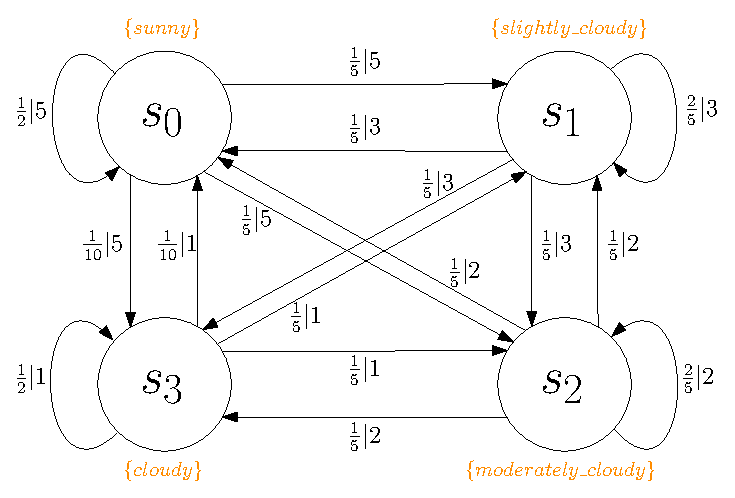
\includegraphics[width=0.6\linewidth]{resources/weather-solar-pannel}
    \caption{MC modeling a daily production of energy (in $kJ$) of solar pannels according to weather}
    \label{MCexample}
  \end{figure}
  The way $w$ is defined for this MC yields that when a day is sunny, the installation produces $5 kJ$ during this day, $3 kJ$ when a day is slightly cloudy, $2 kJ$ when a day is moderately cloudy and finaly $1 kJ$ when the day is cloudy.
\end{example}
